\documentclass[a4paper,twoside,12pt]{report}
% Richard Klein (2020,2021)
% Content: Sachin Mohan (2026)

% Include Packages
%\usepackage[a4paper,inner=3.5cm,outer=2.5cm,top=2.5cm,bottom=2.5cm]{geometry}
\usepackage{fullpage}
\usepackage{float}
\usepackage{url}
\usepackage{charter}
\usepackage{graphicx}
\graphicspath{{../}}
\usepackage{subfigure}
\usepackage{amsmath}
\usepackage{amssymb}
\usepackage{amsthm}
\usepackage{booktabs}
\usepackage{parskip}
\usepackage[all]{nowidow}
\setnoclub[2]
\setnowidow[2]
\usepackage{pdfpages}

% Allow LaTeX more slack to resolve overfull lines without manual breaks
\emergencystretch=3em
\hbadness=10000
\vbadness=10000
\hfuzz=2pt
\vfuzz=2pt

% Referencing
\usepackage{varioref}
\usepackage[bookmarks=true,bookmarksopen=true]{hyperref}
\usepackage{cleveref}
\hypersetup{
  colorlinks   = true,
  urlcolor     = blue,
  linkcolor    = blue,
  citecolor    = blue
}
\crefname{table}{table}{tables}
\Crefname{table}{Table}{Tables}
\crefname{figure}{figure}{figures}
\Crefname{figure}{Figure}{Figures}
\crefname{equation}{equation}{equations}
\Crefname{equation}{Equation}{Equations}

% Wits Citation Style
\usepackage{natbib} \input{natbib-add}
\bibliographystyle{named-wits}
\bibpunct{[}{]}{;}{a}{}{}
\setlength{\skip\footins}{1.5cm}
\newcommand{\citets}[1]{\citeauthor{#1}'s \citeyearpar{#1}}
\renewcommand\bibname{References}

\pagestyle{headings}
\pagestyle{plain}
\pagenumbering{roman}

\renewenvironment{abstract}{\ \vfill\begin{center}\textbf{Abstract}\end{center}\addcontentsline{toc}{section}{Abstract}}{\vfill\vfill\newpage}
\newenvironment{declaration}{\ \vfill\begin{center}\textbf{Declaration}\end{center}\addcontentsline{toc}{section}{Declaration}}{\vfill\vfill\newpage}
\newenvironment{acknowledgements}{\ \vfill\begin{center}\textbf{Acknowledgements}\end{center}\addcontentsline{toc}{section}{Acknowledgements}}{\vfill\vfill\newpage}

\begin{document}
\onecolumn
\thispagestyle{empty}

\setcounter{page}{0}
\addcontentsline{toc}{chapter}{Preface}
\

\begin{center}
  \vfill
  {
  \huge \bf \textsc{Evolutionary Multi-Objective Planning in Joint-Embedding Predictive Architectures for Safe Reinforcement Learning}\\[10pt]
  \large Selection Pressure as an Alternative to Hand-Crafted Reward Penalties\\[20pt]
  \large School of Computer Science \& Applied Mathematics\\
  \large University of the Witwatersrand\\[20pt]
  \normalsize
  Sachin Mohan\\
  2699183\\[20pt]
  Supervised by Geraud Nangue Tasse\\[10pt]
  \today
  }

  \vfill
  \vfill
  
\includegraphics[width=1.5cm]{images/wits}
  \vspace{10pt}\\
  \small{A proposal submitted to the Faculty of Science, University of the Witwatersrand, Johannesburg,
in partial fulfilment of the requirements for the degree of Bachelor of Science with Honours}\\
\end{center}
\vfill
\newpage

\pagestyle{plain}
\setcounter{page}{1}

% =====================================================
% ABSTRACT
% =====================================================
\phantomsection
\begin{abstract}
Safe reinforcement learning (RL) seeks to train agents whose behaviour respects safety constraints during both learning and deployment stages. The dominant approaches rely on hand-crafted reward penalties or explicit cost functions, both of which are fragile: small changes to penalty weights produce either reckless or paralysed agents, and writing a good cost function is often as hard as writing the reward. This work proposes an alternative grounded in \emph{selection pressure} rather than reward shaping. A Joint-Embedding Predictive Architecture (JEPA) world model is proposed to be paired with a multi-objective evolutionary planner that searches over action sequences in the model's latent space. Instead of a single designed cost function, the planner uses \emph{structural} safety signals that come for free from the world model itself. It returns not a single best plan but a Pareto front of trade-offs between task performance and safety, letting the operator choose how cautious the agent should be at deployment rather than fixing this in advance. The framework will be evaluated on the Push-T, Reacher, and OGBench-Cube benchmarks against standard penalty-tuned and constrained-RL baselines, with controlled perturbations used to test whether the model's own prediction error is a reliable indicator of unsafe situations. If successful, this removes the need for engineers to guess the right safety-performance trade-off in advance: the trade-off becomes a deployment-time choice. More broadly, it asks whether selection pressure can substitute for the hand-tuned reward engineering that current safe-RL methods depend on.
\end{abstract}

% =====================================================
% DECLARATION
% =====================================================
\phantomsection
\begin{declaration}
I, Sachin Mohan (Student Number: 2699183), hereby declare the contents of this research proposal to be my own work.
This proposal is submitted for the degree of Bachelor of Science with Honours in Computer Science at the University of the Witwatersrand.
This work has not been submitted to any other university, or for any other degree.
\end{declaration}

\phantomsection
\addcontentsline{toc}{section}{Table of Contents}
\tableofcontents
\newpage
\phantomsection
\addcontentsline{toc}{section}{List of Figures}
\listoffigures
\vspace{1.5cm}
\phantomsection
\addcontentsline{toc}{section}{List of Tables}
\begingroup
  \let\clearpage\relax
  \let\cleardoublepage\relax
  \listoftables
\endgroup
\newpage
\pagenumbering{arabic}

% =====================================================
% CHAPTER 1: INTRODUCTION
% =====================================================
\chapter{Introduction}

Reinforcement learning (RL) has produced remarkable advances in agents that learn complex behaviour from interaction, from mastering board games like GO\citep{silver2017alphazero} to controlling robotic systems \citep{kalashnikov2018qtopt} and powering large language models \citep{ouyang2022instructgpt}. Agents have moved from simulated environments toward physical deployment, and so ensuring that they behave \emph{safely} becomes a big concern. For example a robot that learns to manipulate objects must not damage them or the people around it. And so the question is not whether RL agents should be safe, but how safety should be expressed in their training objectives?

The predominant approach is \emph{reward shaping}: the task reward is augmented with a penalty term that discourages unsafe states or actions. However this approach is conceptually simple but practically fragile. If the penalty weight is too small, the agent learns to ignore it and behaves unsafely; if it is too large, the agent becomes paralysed and refuses to act at all. The ``correct'' weight depends on environment dynamics, task structure, and the relative scales of reward and cost, quantities the system designer rarely knows in advance \citep{skalse2022rewardhacking,fu2025rewardshaping}. Constrained reinforcement learning approaches \citep{achiam2017cpo,ray2019safetygym} formalise safety as an explicit constraint rather than a penalty, but transfers the problem rather than solving it: instead of designing a reward, the engineer must design a cost function and a constraint threshold, both of which suffer from the same specification difficulties.

Biology suggests an alternative: animals that act unsafely do not survive, so the constraint is enforced implicitly. This research builds on this idea and investigates whether \emph{evolutionary} rather than reward-based mechanisms can produce safe behaviour without explicit penalty engineering. The core idea is to abandon scalarising the reqrd entirely. Rather than collapsing reward and safety into a single objective with a chosen weight, treat them as separate axes and search for the Pareto front of trade-offs. The operating point is selected at deployment, not engineered into training.

Multi-objective evolutionary algorithms such as NSGA-II \citep{deb2002nsga2} are natural tools for this approach, but applying them to high-dimensional control problems involves evaluating each candidate and requires costly environment rollouts, and unsafe candidates may need to be evaluated in the real world to be detected. This research proposes to combine evolutionary multi-objective planning with a learned world model based on the Joint-Embedding Predictive Architecture (JEPA) framework \citep{lecun2022path,maes2026lewm}. JEPA models predict future states in a compact latent space rather than reconstructing pixels, learning task-agnostic dynamics from offline data without reward supervision. Evolutionary search occurs entirely in this latent space, evaluating thousands of candidate plans cheaply before any are executed in the real world.

\Cref{fig:system} gives a high-level overview of the proposed pipeline. Observations are encoded by a frozen JEPA encoder into a latent representation; an NSGA-II planner maintains a population of candidate action sequences, which are rolled out in latent space by the JEPA predictor; structural safety objectives are computed along each imagined trajectory; the planner returns a Pareto front of plans trading off task achievement and safety; a deployment-time selector picks the operating point; and the first $k$ actions of the chosen plan are executed under model predictive control before replanning.

\begin{figure}[ht]
    \centering
    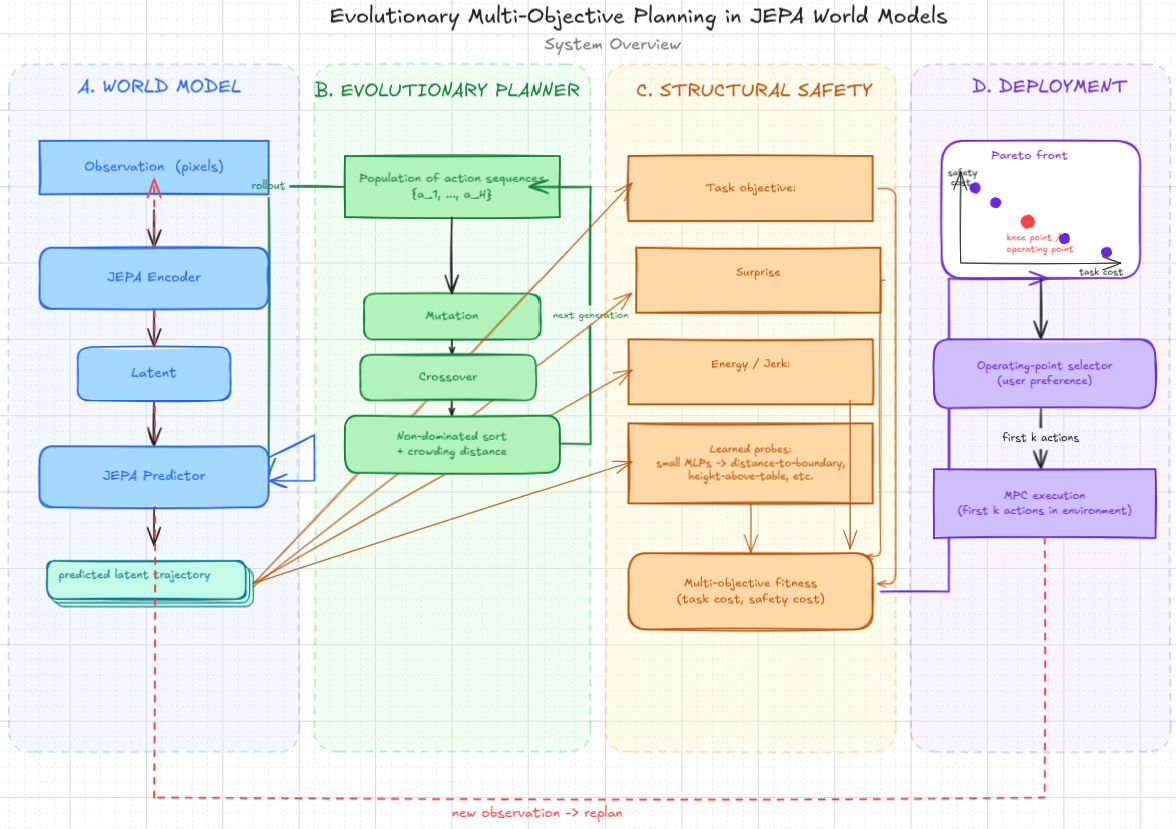
\includegraphics[width=0.98\linewidth]{images/full_system}
    \caption[Pipeline overview.]{Overview of the proposed pipeline.}
    \label{fig:system}
\end{figure}

% =====================================================
% CHAPTER 2: BACKGROUND AND RELATED WORK
% =====================================================
\chapter{Background and Related Work}\label{ch:background}

\section{Reinforcement Learning}

Reinforcement learning is formalised as a Markov Decision Process $(S, A, P, R, \gamma)$ in which the agent learns a policy $\pi(a|s)$ maximising the expected discounted return $\mathbb{E}[\sum_t \gamma^t R(s_t, a_t)]$ \citep{sutton2018rl,puterman2014mdp}. Deep RL approximates $\pi$ with neural networks, enabling learning from high-dimensional observations such as images \citep{mnih2013atari,haarnoja2018sac}. The goal-conditioned variant $\pi(a|s, g)$ \citep{ghosh2019goal} is well suited to the manipulation tasks studied here, where many tasks share dynamics but differ in their target configurations.

\section{Safe Reinforcement Learning}

\citet{garcia2015survey} survey two main families of safe RL. The first \emph{modifies the reward} with a penalty $R'(s,a) = R(s,a) - \lambda C(s,a)$; the second \emph{imposes explicit constraints} via Constrained Policy Optimisation \citep{achiam2017cpo} or Lagrangian PPO. Both require the designer to specify a cost function $C$, which is often as hard as designing the reward \citep{skalse2022rewardhacking,fu2025rewardshaping}; attempts to derive $C$ from large language models \citep{kwon2023reward,yu2023languagerewards} inherit the limitations of their oracles. An alternative is \citet{nanguetasse2024rosarl}'s ROSARL, a reward-only framework that derives the smallest provably-safe penalty from intrinsic environment quantities (diameter and controllability) and outperforms CPO and TRPO-Lagrangian on stochastic benchmarks; although still single-objective, its core insight aligns with the structural-safety view taken here. Empirical comparison is standardised by Safety-Gymnasium \citep{ji2023safetygym} and its SafePO library of 16 baselines; extension to those environments is a follow-up identified in \Cref{ch:methodology}. \emph{Model-based} safe RL evaluates candidate actions in imagination, with model-accuracy concerns increasingly addressed by world models that expose explicit out-of-distribution signals \citep{garrido2025intuitive}.

\section{World Models and Joint-Embedding Predictive Architectures}

World models predict environment dynamics \citep{ha2018worldmodels} with generative variants reconstructing future pixels \citep{hafner2020dreamer,hafner2023dreamerv3} but this commits substantial capacity to visual detail irrelevant to control. Joint-Embedding Predictive Architectures (JEPAs), proposed by \citet{lecun2022path}, instead predict future \emph{latents} conditioned on actions (\Cref{fig:jepa}) The prediction loss is computed in latent space, freeing the model from rendering the world. JEPA training has been applied to image \citep{assran2023ijepa} and video \citep{bardes2024vjepa} representation learning, and recently to action-conditioned world models for control \citep{sobal2025stresstest,zhou2025dinowm,maes2026lewm}.

\begin{figure}[ht]
    \centering
    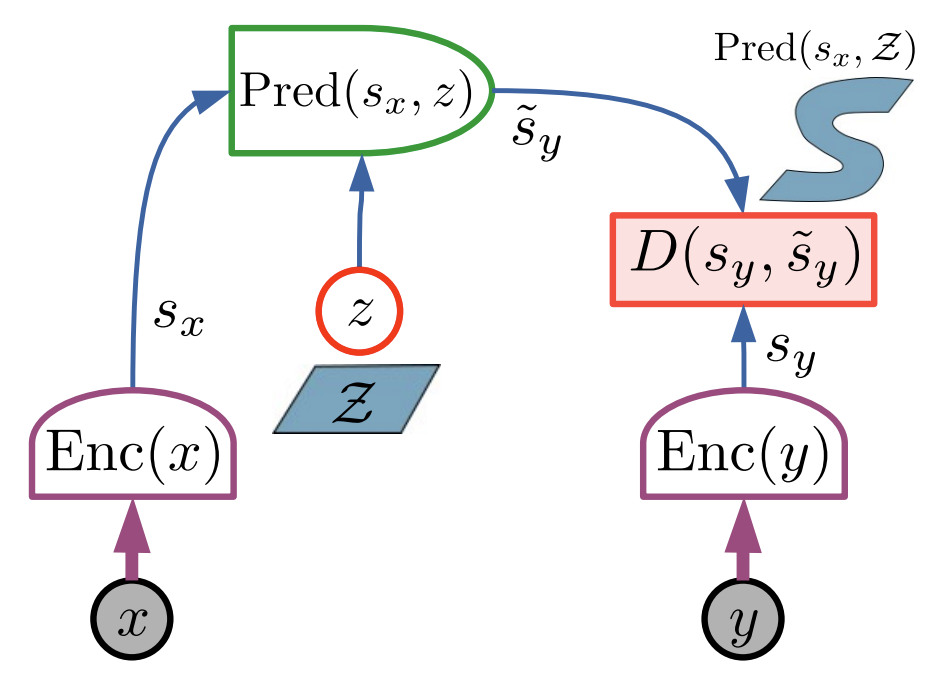
\includegraphics[width=0.55\linewidth]{images/lv_jepa}
    \caption[JEPA architecture.]{Schematic of a Joint-Embedding Predictive Architecture. An encoder maps the observation $s_t$ to a latent $z_t$; conditioned on an action $a_t$, a predictor produces $\hat{z}_{t+1}$. The prediction loss is computed in latent space rather than at the pixel level, allowing the model to discard control-irrelevant visual detail.}
    \label{fig:jepa}
\end{figure}

A central challenge in JEPA training is \emph{representation collapse} (the trivial mapping of all inputs to a constant), addressed by stop-gradient updates \citep{assran2023ijepa,bardes2024vjepa}, frozen pre-trained encoders \citep{zhou2025dinowm}, or variance-covariance regularisation \citep{bardes2022vicreg,sobal2025stresstest}. LeWM \citep{maes2026lewm} introduces the Sketched Isotropic Gaussian Regulariser (SIGREG) \citep{balestriero2025lejepa}, achieving provably stable end-to-end training from pixels with a single effective hyperparameter, and additionally shows that JEPA latents support linear probes for physical quantities, prediction surprise as an out-of-distribution flag, and cross-entropy planning \citep{rubinstein2004ce} competitive with foundation-model-based methods. This research builds directly on LeWM as the world-model substrate.

\section{Evolutionary Computation and Multi-Objective Optimisation}

Evolutionary algorithms are population-based, gradient-free optimisers \citep{eiben2015evolutionary}. In policy search, evolution strategies \citep{salimans2017es}, neuroevolution \citep{such2017neuroevolution}, and cross-entropy methods (CEM) \citep{rubinstein2004ce} are competitive with gradient-based RL on continuous control. CEM, the planner used in LeWM, is a simple evolutionary procedure: sample action sequences from a Gaussian, evaluate, select elites, refit. It converges to a single optimum and does not natively handle multiple objectives.

Quality-Diversity (QD) algorithms such as MAP-Elites \citep{mouret2015mapelites} preserve diverse archives of solutions indexed by behavioural descriptors, and have been extended to RL by \citet{tjanaka2022dqdrl}, who note that the advantage of differentiable QD methods diminishes when gradients must be approximated from rollouts. Multi-objective evolutionary algorithms (MOEAs) such as NSGA-II \citep{deb2002nsga2} take a different tack: rather than scalarising, they maintain a Pareto front of non-dominated solutions, where $x$ dominates $x'$ if $f_i(x) \leq f_i(x')$ for all $i$ with strict inequality in at least one \citep{miettinen1999nonlinear}. NSGA-II uses non-domination ranking and crowding distance to balance convergence and diversity, and scales well to two-to-four objectives; higher-dimensional objective spaces require NSGA-III \citep{deb2014nsga3}. The objective space here is two-dimensional (task achievement and safety), so NSGA-II suffices, and its gradient-free design sidesteps the QD-RL pitfall identified by \citet{tjanaka2022dqdrl}. Both QD and MOEA approaches have been applied to safe RL in limited form \citep{sobal2025stresstest,mouret2023qdsafety} but, to the author's knowledge, never with a JEPA-style world model.

\section{Synthesis and Research Gap}\label{sec:gap}

Three strands of recent work motivate this proposal. JEPA-style world models \citep{lecun2022path,maes2026lewm,zhou2025dinowm} learn task-agnostic latent dynamics and expose intrinsic signals such as prediction surprise that serve as out-of-distribution detectors. Multi-objective evolutionary algorithms \citep{deb2002nsga2} produce Pareto fronts without requiring a scalar weight. Structural safety signals derived from a learned model \citep{garrido2025intuitive,maes2026lewm} sidestep the cost-function specification problem that limits both penalty-based and constrained-RL approaches \citep{achiam2017cpo,skalse2022rewardhacking}. Existing safe-RL methods occupy parts of this space individually (hand-crafted penalties \citep{garcia2015survey,achiam2017cpo}, principled but still single-objective reward shaping \citep{nanguetasse2024rosarl}, or multi-objective search in policy space without a model-based safety substrate \citep{mouret2023qdsafety,tjanaka2022dqdrl}), but none combines all three. The contribution of this proposal lies in that intersection: using JEPA's intrinsic signals as the safety axis and an evolutionary planner to expose the resulting trade-off as a Pareto front.

% =====================================================
% CHAPTER 3: RESEARCH OBJECTIVES
% =====================================================
\chapter{Research Objectives}\label{ch:objectives}

This chapter states the goals of the research and the central hypotheses that will be empirically tested.

\section{Research Question}

This research asks a single central question: \emph{can a multi-objective evolutionary planner operating in the latent space of a JEPA world model, using only structural safety signals derived from the model itself, recover safety-performance trade-offs that are competitive with hand-tuned penalty-based methods and constrained reinforcement learning?}

\section{Research Goals}

The primary goals of this research are as follows.

\paragraph{1. Evolutionary Planning in Latent Space.} Develop a multi-objective evolutionary planner based on NSGA-II that operates over action sequences in the latent space of a JEPA world model, returning a Pareto front of plans trading off task achievement against predicted safety violations.

\paragraph{2. Structural Safety Objectives.} Develop a suite of safety signals derived from intrinsic properties of the world model rather than from hand-crafted cost functions. Specifically: prediction surprise as an out-of-distribution detector; latent energy and jerk as smoothness signals; and small learned probes for specific safety-relevant quantities.

\paragraph{3. Empirical Comparison Against Penalty-Tuned Baselines.} Demonstrate that the proposed framework achieves competitive or superior safety-performance trade-offs compared to cross-entropy planning with hand-tuned safety penalties and against constrained reinforcement learning baselines, on standard goal-conditioned control benchmarks (Push-T, Reacher, OGBench-Cube).

\paragraph{4. Characterisation of Surprise-Based Safety.} Empirically characterise the conditions under which JEPA prediction surprise serves as a reliable safety proxy, using a violation-of-expectation framework with controlled perturbations. The aim is not to claim that surprise is always safety-correlated but to identify when it is and is not.

\section{Research Hypotheses}

The central hypotheses of this research are as follows.

\begin{itemize}
    \item \textbf{H1:} A multi-objective evolutionary planner operating in JEPA latent space can recover a Pareto front of plans whose performance points dominate or match those produced by cross-entropy method planning with hand-tuned safety penalties, across a range of penalty values.

    \item \textbf{H2:} Prediction surprise in a stably trained JEPA world model correlates reliably with physical violations (object teleportation, abrupt state changes) but less reliably with purely visual perturbations (colour changes, lighting shifts), as suggested by prior violation-of-expectation results \citep{maes2026lewm}.

    \item \textbf{H3:} Combining multiple structural safety objectives (surprise, energy, learned probes) produces a more robust safety axis than any single signal alone, with decreasing marginal benefit as additional signals are added.

    \item \textbf{H4:} The resulting framework is comparable in safety-performance trade-off to constrained RL baselines (CPO, Lagrangian PPO) while requiring no manual specification of a cost function or constraint threshold.
\end{itemize}

% =====================================================
% CHAPTER 4: RESEARCH METHODOLOGY
% =====================================================
\chapter{Research Methodology}\label{ch:methodology}

The research is organised into four sequential phases, each building on the outputs of the previous one. Phases 1 and 2 establish the technical substrate (world model and planner); Phase 3 introduces the core safety contributions; Phase 4 produces the main empirical comparisons. Phases are designed so that the project can be pruned to a shorter form (Phases 1--3 only) if time pressure requires, while preserving a coherent contribution.

\section{Phase 1: JEPA World Model Reproduction}

The first phase establishes the world model substrate by reproducing LeWM \citep{maes2026lewm} on the Reacher and Push-T environments. This phase serves two purposes: it provides the trained world model used in subsequent phases, and it verifies that the codebase and infrastructure are working before more substantive contributions are attempted. The three environments used across the project are shown in \Cref{fig:envs}.

\begin{figure}[ht]
    \centering
    \subfigure[Reacher]{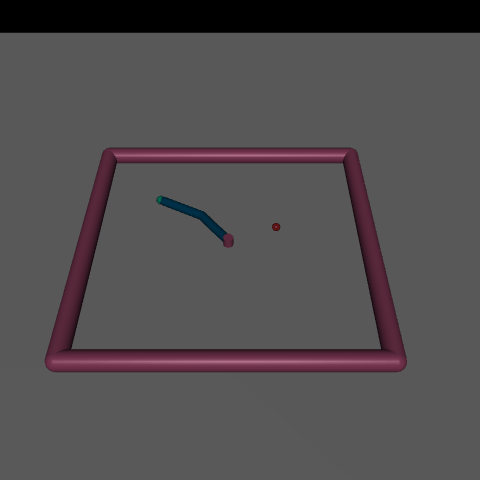
\includegraphics[width=0.30\linewidth]{images/reacher}\label{fig:env-reacher}}
    \hfill
    \subfigure[Push-T]{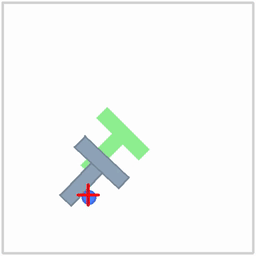
\includegraphics[width=0.30\linewidth]{images/pusht}\label{fig:env-pusht}}
    \hfill
    \subfigure[OGBench-Cube]{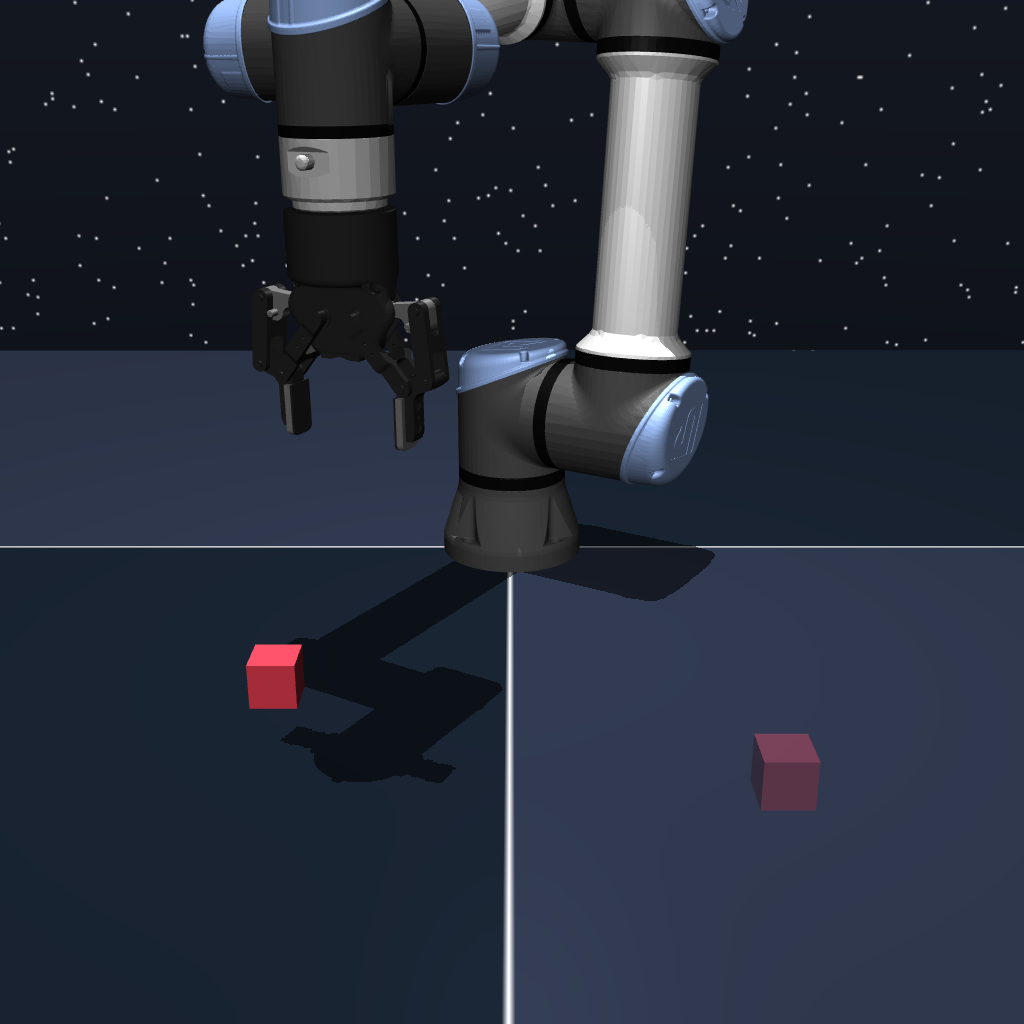
\includegraphics[width=0.30\linewidth]{images/og-cube}\label{fig:env-ogcube}}
    \caption[Evaluation environments.]{Evaluation environments. Reacher (a two-link arm reaching a target) and Push-T (an agent pushing a T-shape into a goal outline) are the primary benchmarks used for LeWM reproduction and planner comparison. OGBench-Cube serves as a generalisation test if time permits.}
    \label{fig:envs}
\end{figure}


Reproduction will use the open-source \emph{stable-worldmodel} framework \citep{maes2026lewm}. Success is measured by matching the published planning success rates on Reacher and Push-T ($\approx$96\% and $\approx$90\% respectively). Once reproduction is verified, the trained world model is frozen and used as the substrate for all subsequent experiments.

\section{Phase 2: Multi-Objective Evolutionary Planning}

The second phase replaces LeWM's cross-entropy method (CEM) planner with a multi-objective evolutionary planner based on NSGA-II. Each candidate is a sequence of actions of a fixed planning horizon; its fitness is evaluated by rolling the sequence through the frozen JEPA predictor and scoring the resulting latent trajectory against two separate objectives, namely a task objective (latent distance to the goal at the terminal step) and a safety objective developed in Phase~3. Rather than combining these into a single scalar reward, NSGA-II returns a Pareto front of non-dominated plans; the operating point is selected at deployment time, not committed to during search.

The substitution from CEM to NSGA-II is performed in two steps to manage risk.

\paragraph{Step 1: Single-objective NSGA-II.} Implement NSGA-II as a drop-in replacement for CEM, optimising only the task achievement objective. Variation operators are Gaussian mutation and crossover at action boundaries. Verification: NSGA-II should produce task success rates within a small margin of CEM on the baseline Push-T and Reacher tasks, confirming that the substitution does not regress task performance.

\paragraph{Step 2: Multi-objective NSGA-II.} Extend NSGA-II to both objectives. The algorithm returns a Pareto front rather than a single optimum. At deployment, the operating point is selected by a user-specified preference (for example, the highest task-performance plan whose predicted safety cost is below a threshold) or by a default policy of selecting the knee point of the Pareto front.

Model Predictive Control (MPC) execution follows LeWM: only the first few actions of the chosen plan are executed before the planner is re-invoked from the new observation. This receding-horizon scheme bounds the accumulation of prediction errors that would otherwise compound over long open-loop rollouts.

\section{Phase 3: Structural Safety Objectives}

The third phase develops the safety objectives that feed into the multi-objective planner. Three signals are proposed, none of which requires manual specification of a cost function.

\paragraph{Surprise.} The prediction error along an imagined rollout, summed across the trajectory, is taken as an out-of-distribution detector. High surprise indicates that the rollout has visited states the model is uncertain about, which is a reasonable proxy for risk. This is the same signal that LeWM uses in its violation-of-expectation evaluation.

\paragraph{Energy and jerk.} The magnitude of consecutive latent differences (and changes in those differences) provides a smoothness signal. High latent velocity or rapid changes in latent velocity, called jerk, indicate sudden, potentially unsafe motion in the underlying physical state. Unlike penalty-based smoothness terms, this signal does not require choosing a weight; it enters the multi-objective optimisation as a separate axis.

\paragraph{Learned probes.} Small multi-layer perceptrons are trained to extract specific safety-relevant quantities from latent embeddings. For example, for the Push-T environment a probe might predict ``distance from the agent to the workspace boundary''; for OGBench-Cube it might predict ``height of the cube above the table surface''. Probes are trained on a small labelled subset of the offline dataset (the labels being computed directly from the simulator state, which is available during training but not during deployment). At deployment, probe outputs along a rollout contribute to the safety objective.

Crucially, the choice of which quantity a probe extracts is not a hand-crafted cost function in the same sense as a penalty term. The probe extracts a structural property of the environment that the engineer regards as \emph{observable} and \emph{relevant}, but the safety \emph{trade-off} between this property and task performance is never specified by the engineer. The Pareto front of the multi-objective optimisation makes the trade-off explicit and selectable at deployment time.

\section{Phase 4: Evaluation and Optional Extensions}

The fourth phase produces the empirical evaluation that tests the central hypotheses.

\paragraph{Baseline comparison.} Four baselines are compared against the proposed method on each of three environments (Push-T, Reacher, OGBench-Cube): (i) vanilla CEM planning, as in LeWM, without any safety consideration; (ii) CEM with hand-tuned safety penalties added to the cost function, swept across a range of penalty weights to recover an empirical Pareto front; (iii) a constrained reinforcement learning baseline, either Constrained Policy Optimisation \citep{achiam2017cpo} or a Lagrangian variant of PPO; and (iv) ROSARL \citep{nanguetasse2024rosarl}, which represents the reward-only paradigm by deriving a principled Minmax penalty from intrinsic environment quantities rather than from hand tuning. Comparing against (iv) is particularly informative because it isolates the contribution of the multi-objective framing: ROSARL and the proposed method both avoid hand-crafted penalties, but ROSARL still commits to a single scalar reward whereas the proposed method exposes the trade-off as a Pareto front. The proposed method's Pareto front is compared against the front recovered from baseline (ii) using hypervolume and inverted generational distance metrics \citep{riquelme2015performance}.

\paragraph{Violation-of-expectation evaluation.} Following LeWM, controlled perturbations are injected into trajectories during evaluation: a physical perturbation in which an object is teleported to a random location, and a visual perturbation in which an object's colour changes abruptly. The framework's surprise signal should spike at the moment of physical perturbation, triggering a fallback to a more conservative plan along the Pareto front. This experiment tests Hypothesis H2.

\paragraph{Ablations.} The contribution of each safety signal (surprise, energy, probe) is isolated by running the framework with each signal alone and with different combinations. This tests Hypothesis H3 about the relative and combined value of structural safety signals.

\paragraph{Optional extensions (if time permits).} Two extensions are identified as natural follow-ups should the core phases complete ahead of schedule: (i) value-function bootstrapping for longer-horizon planning, in the style of TD-MPC2 \citep{hansen2024tdmpc2}, where a learned value function $V(z)$ is used as a terminal cost beyond the planning horizon, and (ii) MAP-Elites style quality-diversity search, where JEPA latent embeddings of trajectories serve as the behavioural descriptor \citep{mouret2015mapelites}. Both extensions are scoped as deferrable contributions to manage project risk.

% =====================================================
% CHAPTER 5: RESEARCH PLAN
% =====================================================
\chapter{Research Plan}\label{ch:plan}

\section{Time Plan}

The project will run from May 2026 to November 2026 (approximately seven months). The compressed schedule is deliberately front-loaded with infrastructure work, and the methodology to take advantage of the holiday period. If any phase overruns, the optional extensions and the third evaluation environment (OGBench-Cube) will be dropped first.

\begin{table}[ht]
\centering
\caption[Project timeline.]{Project timeline (May 2026 -- November 2026). Each phase produces concrete deliverables that can be reviewed before the next phase begins.}
\label{tab:timeplan}
\begin{tabular}{@{}llp{9cm}@{}}
\toprule
\textbf{Phase} & \textbf{Period} & \textbf{Activities} \\
\midrule
Phase 1 & May -- mid-June       & Set up development environment; reproduce LeWM on Reacher (and Push-T if time allows); verify published benchmarks. \\
Phase 2 & mid-June -- mid-July  & Implement single-objective NSGA-II planner; verify parity with CEM on baseline tasks; extend to multi-objective. \\
Phase 3 & mid-July -- August    & Develop and validate the structural safety suite (surprise, energy, probes); integrate into multi-objective planner. \\
Phase 4 & September -- October  & Run main empirical comparison against baselines; violation-of-expectation experiments; ablation studies. \\
Write-up & November             & Analysis, final experiments suggested by results, thesis writing, supervisor revisions, submission. \\
\bottomrule
\end{tabular}
\end{table}

\section{Success Criteria}

The research will be evaluated against the following criteria, in order of decreasing necessity. Criteria (a) and (b) are required for a defensible thesis; criterion (c) is the headline empirical contribution; criterion (d) is a strong addition.

\begin{itemize}
    \item[(a)] Reproducible LeWM training on at least one environment, matching published task success within 5\%.
    \item[(b)] A working multi-objective planner that recovers, at minimum, the same Pareto front as penalty-tuned CEM swept across penalty weights.
    \item[(c)] Empirical demonstration that structural safety objectives (without hand-crafted cost functions) produce a Pareto front comparable to or better than hand-tuned baselines.
    \item[(d)] A characterisation experiment identifying when surprise-based safety is and is not reliable, drawing on the violation-of-expectation framework.
\end{itemize}

\section{Possible Challenges}

Several risks could affect the timeline or scope of the project. They are listed with mitigation strategies.

\paragraph{Reproduction overruns.} Reproducing LeWM on a non-trivial environment may take longer than the six weeks allocated to Phase 1 due to infrastructure issues (CUDA, MuJoCo, Gymnasium compatibility). \emph{Mitigation:} begin with Reacher (the simplest published environment) and target Push-T only once Reacher is working. If reproduction stalls past mid-July, the project can fall back to using the frozen DINO-WM encoder \citep{zhou2025dinowm} as a substrate, preserving the multi-objective planning contribution at the cost of the end-to-end story.

\paragraph{Probe quality.} If learned safety probes do not extract their target quantities cleanly, the safety axis becomes noisy. \emph{Mitigation:} start with surprise alone, which is model-intrinsic and requires no probe training. Add probes incrementally only after the surprise-only baseline is working.

\paragraph{Surprise is not always safety.} Some safety violations may have low surprise (the model can be confidently wrong about dynamics). \emph{Mitigation:} this is treated as a research finding rather than a failure. The characterisation experiment (Goal 4) is explicitly designed to identify these regimes.

\paragraph{Computational budget.} Multi-objective evolutionary planning is more expensive than CEM, and the experimental matrix grows quickly with number of safety signals and environments. \emph{Mitigation:} restrict the main comparison to two environments (Reacher and Push-T) and treat OGBench-Cube as a generalisation test if time permits. Pre-compute world-model rollouts where possible.

% =====================================================
% CHAPTER 6: CONCLUSION
% =====================================================
\chapter{Conclusion}\label{ch:conclusion}

This proposal has outlined a research project investigating whether evolutionary multi-objective optimisation, combined with a JEPA world model and structural safety objectives, can produce safe reinforcement learning behaviour without the fragile hand-crafted reward penalties or cost functions that current methods rely on. The central contribution is methodological: by framing safety as a separate axis in a Pareto-front optimisation rather than as a scalar penalty, the project removes the need for designers to specify a safety-performance trade-off in advance. The trade-off becomes a deployment-time decision over the recovered front.

The framework integrates three lines of recent work that have not previously been combined: LeWM's stable end-to-end JEPA training \citep{maes2026lewm}, NSGA-II multi-objective optimisation \citep{deb2002nsga2}, and intrinsic-model safety signals such as prediction surprise \citep{garrido2025intuitive}. The synthesis is designed to inherit the strengths of each: JEPA's task-agnostic dynamics and free OOD signal, NSGA-II's principled multi-objective handling, and structural safety's independence from hand-crafted cost functions.

If successful, the project demonstrates a small but meaningful step toward safe AI systems that do not depend on engineers correctly anticipating every safety trade-off in advance. More ambitious extensions (hierarchical world models for longer-horizon safety guarantees, quality-diversity over policies, end-to-end co-evolution of model and planner) are explicitly out of scope for the honours project but are positioned as natural follow-up work at master's and doctoral scale.

% =====================================================
% BIBLIOGRAPHY
% =====================================================
\bibliography{references}\addcontentsline{toc}{chapter}{References}

% =====================================================
% AI DECLARATION (appended as final pages)
% =====================================================
\includepdf[pages=-]{../AI_Declaration.pdf}

\end{document}
